\documentclass[12pt,letterpaper]{article}
\usepackage[utf8]{inputenc}
\usepackage{kpfonts}
\usepackage[T1]{fontenc}

% custom titles
\usepackage{titlesec}

% fix broken title numbering with 2016 titlesec update
\usepackage{etoolbox}

\makeatletter
\patchcmd{\ttlh@hang}{\parindent\z@}{\parindent\z@\leavevmode}{}{}
\patchcmd{\ttlh@hang}{\noindent}{}{}{}
\makeatother
%%%

\titlespacing*\section{0pt}{12pt plus 4pt minus 2pt}{0pt plus 2pt minus 2pt}
\titlespacing*\subsection{0pt}{12pt plus 4pt minus 2pt}{0pt plus 2pt minus 2pt}
\titlespacing*\subsubsection{0pt}{12pt plus 4pt minus 2pt}{0pt plus 2pt minus 2pt}

% Package for double spacing
\usepackage{setspace}
\usepackage{ragged2e}

% Set 1.0 inch margins
\usepackage[margin=1.0in, headheight=15pt]{geometry}
\usepackage{enumitem}

% Use images and graphics
\usepackage{graphicx}
\usepackage{float}

% Use nicer headers
\usepackage{fancyhdr}
\pagestyle{fancy}
\renewcommand{\headrulewidth}{0pt}
\rhead{CIS3750 - Assignment 2}

% sections should be indexed with alphabets
\renewcommand{\thesection}{\Alph{section}}

%double spaced lines in the whole document
\doublespacing

\title{Assignment 1}

\begin{document}
\begin{titlepage}
    \centering
    \vspace*{\baselineskip}
    \rule{\textwidth}{1.6pt}\vspace*{-\baselineskip}\vspace*{2pt}
    \rule{\textwidth}{0.4pt}\\[1.5\baselineskip]
    {\LARGE \textsc{An Initial Outline of a Software System to Improve Food Security in Malawi}}\\[\baselineskip]
	\rule{\textwidth}{0.4pt}\vspace*{-\baselineskip}\vspace{4pt}    
    \rule{\textwidth}{2pt}\\[2\baselineskip]
   
    \vspace*{5\baselineskip}
    \textsc{BY}\\[0.25\baselineskip]
    {\LARGE HANLON} \\
    
    \vspace*{\baselineskip}
    % List of authors in alphabetical order (by last name)
    {\textsc{David DiMaria \\ Braydon Johnson \\ Joshua Lemieux \\ Neivin Mathew \\ Like Zheng} \par}
    \vfill
    {\scshape October 14, 2016} \\
  \end{titlepage}
  
  
% Table of Contents (no page numbers on contents)
\pagenumbering{roman} %roman numerals for ToC
\tableofcontents
\lhead{} % remove default header from Contents page
\clearpage
\pagenumbering{arabic} %pagenumbering in arabic numbers
    
\section{Client Details}
Malawi is a country located in the warm heart of Africa, with a population of 16.4 million. According to the Malawi Vulnerability Assessment Committee, an estimated 2.83 million people will experience acute food insecurity during the 2015/16 lean season. (World Food Programme, 2016) The economy of the country is based on agriculture. The majority of the people in Malawi are farmers who cultivate tobacco for living. Due to the impact of climate change, decline in global tobacco consumption and the scarcity of food in Malawi, the farmers need to transition to growing different crops. However, since Malawian farmers have been growing tobacco for many generations, the current farmers of the country lack the tools and knowledge required in order to start growing other crops. 

The client for the project is the Agricultural Research and Extension Trust (ARET) of Malawi. They are the premier research institution of Malawi, and are responsible for conducting research and providing technical/extension services on tobacco. The trust was established on September 1, 1995 to foster development and information dissemination for Malawi's tobacco industry. It combined the services of two institutions, the Tobacco Research Institute of Malawi (TRIM) and the Estate Extension Service Trust (EEST), who separately provided research and extension services respectively. (ARET, 2016)

ARET states their new vision is "to be a leading regional centre of excellence in agricultural research and technology dissemination which promotes diversification in the agricultural sector." (ARET, 2016). To accomplish this, they require a software system to collect data on the farmers in Malawi, and distribute research conducted within the organization to the farmers of the country. This project aims to fulfill this need.

\clearpage
\section{Team Details}
\subsection{Team Name}
The team name for the project is "Hanlon."\par
The name is inspired by the eponymous highway that runs through the city of Guelph, and signifies the team's ties to the University of Guelph, as well as the city of Guelph.\\

\begin{figure}[H]
	\centering	
	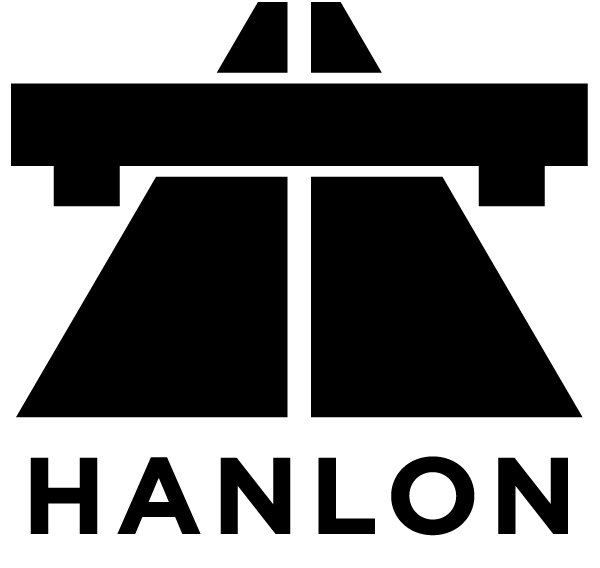
\includegraphics[height=2in]{img/hanlon-logo.png}
	%\caption{The team logo}
	\label{fig:kitten}
\end{figure}

\subsection{Team Members}
Hanlon is comprised of the following students:\\
1. \textbf{\hspace*{5pt} David DiMaria} - Project Manager\\
2. \textbf{\hspace*{5pt}Braydon Johnson} - Software Developer, User Interface Designer\\
3. \textbf{\hspace*{5pt}Joshua Lemieux} - Project Manager, User Interface Designer\\
4. \textbf{\hspace*{5pt}Neivin Mathew} - Software Developer, User Interface Designer\\
5. \textbf{\hspace*{5pt}Like Zheng} - Software Developer

\subsection{Team Roles}
\subsubsection*{Project Manager}
The Project Manager predicts potential problems that may arise during development, and plans tasks to ensure that the project is completed successfully and on time. This role involves the scheduling and unblocking of tasks. It may also involve some programming.

\subsubsection*{Software Developer}
The Developer is involved in all aspects of the software development process including research, design, coding, documentation and testing.

\subsubsection*{User Interface Designer}
The User Interface (UI) Designer role is to plan out and develop any user facing component of the system which includes the specific layout of screens, and improving the interaction between the customer and the product.

\subsection{Team Organization}
Hanlon will follow a static team structure. Each member will maintain their respective roles for the entire duration of the project. \par

Hanlon will use a democratic majority voting system for any decisions that need to be taken within the team. Each present member will be involved in voting, and possesses one vote per motion. A motion is passed when a simple majority is achieved. \par

In the event of a team member being unavailable, and a majority cannot be established, a motion can only be passed through unanimous consent.

\clearpage
\section{Requirements}
\subsection{Definitions}
The terms used in the requirements document are defined as follows:\\
1. \textbf{ARET -- } The Agricultural Research and Extension Trust of Malawi. \\
2. \textbf{SMS -- } Short Message Service. A service on cell phones that allows the exchange of short text messages.\\
3. \textbf{API -- } Application Programming Interface. A set of tools that allows applications to interact with each other.\\
4. \textbf{SQL -- } Structured Query Language. A language that allows the definition and manipulation of data.\\
5. \textbf{GUI -- } Graphical User Interface. A visual framework that enables easy interaction with an application.\\
6. \textbf{System Administrator --} A member of ARET responsible for administering user profiles and maintaining the database and API. They also will have communication with the development team, and report structural changes the database and/or API.\\
7. \textbf{Researcher --} A member of ARET responsible for creating and managing research projects within the system. Additionally, they will be reviewing the materials created by the Extension Officer to make sure they are scientific.\\
8. \textbf{Extension Group --} A member of ARET responsible for using the results from the research projects and creating information that will be disseminated to the farmers from Agents and Officers.\\
9. \textbf{Extension Officer --} A member of ARET responsible for communicating with the Extension Service within the system and disseminating information to their respective Agents.\\
10. \textbf{Extension Agent --} A member of ARET responsible for communicating with their Extension Officer within the system and disseminating information to the Farmers within their region.\\
11. \textbf{Farmer --} A farmer of Malawi responsible for using the mobile application to track their farm statistics, receive notifications from ARET members, and send responses to surveys from ARET.\\
12. \textbf{Public --} Anyone who is using the web application but is not one of the defined users. This could be potential donors, partners etc.\\
13. \textbf{System --} The entire system as a whole, including the web portal, mobile application, database and API.\\
14. \textbf{API Key--}A unique string generated by the system and distributed to an external application, that allows the system to authenticate the application and provide it access to the API.\\
15. \textbf{Notifications --} Push notifications from the system to the mobile application on the user's device.\\
16. \textbf{Field Size --} The length and width of the farmers field. Measured in square meters. \\
17. \textbf{Security criteria --} Constraints that the user's passwords must satisfy, such as the presence of capital letters, or numbers.

\subsection{Multiple Dependencies}
The following requirements have more than one dependency: \\
1. \textbf{Requirement \#027 -} Depends on requirement \#016 and requirement \#013. \\
2. \textbf{Requirement \#029 -} Depends on requirement \#017 and requirement \#013. \\
3. \textbf{Requirement \#030 -} Depends on requirement \#016 and requirement \#014. \\
4. \textbf{Requirement \#035 -} Depends on requirement \#016 and requirement \#015.

\subsection{Requirements Table}
The table of requirements can be found in the file named "\texttt{CIS3750\char`_A2\char`_Hanlon.csv}" file attached to the report.

\clearpage
\section{Use Cases}

\subsection{Upload Research Document for Extension}
\subsubsection*{Primary Actor:} ARET Researcher
\subsubsection*{Stakeholders and Interests:}
1. \emph{ARET Researcher --} wants to upload original research documents to be extended, wants the process to be clear and simple.\\[10pt]
2. \emph{ARET Extension Group --} wants to download original research documents, , wants the process to be clear and simple.

\subsubsection*{Preconditions:}
The researcher is identified and authenticated by the system and has a file ready to be uploaded.

\subsubsection*{Success Guarantee (Postconditions):}
The Researcher successfully uploads a research file to the web portal for the Extension Group to access. List of research files to be extended is updated.

\subsubsection*{Main Success Scenario:}
1. The user indicates to the system that they want to upload a new file for extension.\\
2. The system redirects the user to a page where they are prompted to choose a file from their device or exit the use case \emph{[Use case ends]}.\\
3. The user selects a new file from their device to be uploaded and confirms that the file is correct. \emph{[Alt1: Incorrect file selected]}\\
4. The system validates the selected file on certain criteria such as file format, file size, etc. \emph{[Alt2: file is not correct format][Alt3: file is over size limit]}\\
5. The system uploads the file selected by the user to the system database. 


\subsubsection*{Alternative Flows:}
\emph{Alt1:Incorrect file selected}\\
1. Flow resumes at Main Success Scenario Step 2. \\[10pt]
\emph{Alt2: File is not in correct format}\\
1. The system informs the user that the selected file is of an invalid file format. \\
2. Flow resumes at Main Success Scenario Step 2. \\[10pt]
\emph{Alt3: File exceeds size restriction}\\
1. The system informs the user that the selected file exceeds the size restriction on uploaded files.\\
2. Flow resumes at Main Success Scenario Step 2.


\subsubsection*{Exceptions:}
If at any time the system is unable to authenticate the user, or unable to upload the research document to the database due to failure of the system API or the user’s internet connection, the system informs the user of the problem and the use case ends.


\clearpage
\subsection{View Original Research Document for Extension}
\subsubsection*{Primary Actor:} ARET Extension Group
\subsubsection*{Stakeholders and Interests:}
1. \emph{ARET Extension Group --} wants to download the research data to convert into extension materials, wants accurate research data to convert, wants the process to be clear and simple.\\[10pt]
2. \emph{ARET Researcher --} wants the extension materials generated from the research to accurately convey the research data, wants to know how their research is being used. \\[10pt]
3. \emph{Farmer --} wants the research data to be converted into extension materials, wants to apply the information from the research to their own farm.

\subsubsection*{Preconditions:}
Extension Group member is identified and authenticated by the system.

\subsubsection*{Success Guarantee (Postconditions):}
The Extension Group member successfully downloads a research file from the web portal to their device. The research file data is updated to indicate that it is currently being worked on by the Extension Group.

\subsubsection*{Main Success Scenario:}
1. The user requests a list of research documents that are currently available for conversion to extension materials. \emph{[Alt1: No research documents available]}\\
2. The system retrieves the list of research documents available and displays the list to the user.\\
3. The system provides the user with the choice to select a document or to exit the use case. \emph{[Use case ends]}\\
4. The user selects a research document they want to view.\\
5. The system redirects the user to a page outlining the details of the document (File size, Author, Date of Last Update etc.) \\
6. The user indicates to the system that they would like to either view the selected document, download it to their device \emph{[Alt2: Download research document]}, or select a different research document from the list \emph{[Alt3: Select different research document]}.\\ 
7. The system fetches the document from the ARET database and displays it to the user through their browser.

\subsubsection*{Alternative Flows:}
\emph{Alt1: No research documents available}\\
1. The system informs the user that no research documents are currently available for conversion to extension materials. Use case ends.\\[10pt]
\emph{Alt2: Download research document}\\
1. The system fetches the desired document from the ARET database and downloads the file to the default download directory on the mobile device. \\
2. The system informs the user that the file has been successfully downloaded to the device. \\[10pt]
\emph{Alt3: Select different research document}\\
1. Flow resumes at Main Success Scenario Step 2.

\subsubsection*{Exceptions:}
If at any time the system is unable to authenticate users or retrieve research documents from the system database due to failure of the system API or the user’s internet connection, the system informs the user of the problem and the use case ends.

\clearpage
\subsection{Create a Farmer Account}
\subsubsection*{Primary Actor:} Farmer
\subsubsection*{Stakeholders and Interests:}
1. \emph{Farmer --} wants to create an account, wants to access farming information and research data, wants the process to be clear and simple. \\[10pt]
2. \emph{ARET --} wants the system to correctly record farmer account creation for accurate data collection.
\subsubsection*{Preconditions:}
The mobile application must be built and the API for user creation must be stable.

\subsubsection*{Success Guarantee (Postconditions):}
The Farmer is aware that their account has been created. The user database is updated. Farmer is able to login and access the mobile application content.

\subsubsection*{Main Success Scenario:}
1. The user indicates to the System that they would like to create an account.\\
2. The system verifies that the mobile device is in Malawi to prevent abuse of the System. \emph{[Alt1: Mobile device is not in Malawi]}\\
3. The system redirects the user to an account creation page where they enter in the required information that they are prompted for, and indicate to the System when they are finished creating an account. The user can choose to cancel the creation process and exit the use case. \emph{[Use Case Ends]}\\
4. The system validates the new account information and then returns a message to the user that their account has been created. \emph{[Alt2: Account name fails validation][Alt3: Account password fails validation]}\\
5. The user is redirected to the main application dashboard by the system.

\subsubsection*{Alternative Flows:}
\emph{Alt1: Mobile device is not in Malawi}\\
1.  The system informs the user that their location is invalid and are unable to create an account. \\
2. The system reminds the user to turn on their location services. Use case ends.\\[10pt]
\emph{Alt2: Account name fails validation}\\
1. The system informs the user that their account name either already exists or contains invalid characters. \\
2. Flow resumes at Step 3. \\[10pt]
\emph{Alt3:  Account password fails validation}\\
1. The system informs the user that their account password contains invalid characters or does not meet the criteria for a secure password.
2. Flow resumes at Step 3.

\subsubsection*{Exceptions:}
If at any time the system is unable to call the API, or the user’s internet connection fails, the system informs the user of the problem, and the use case ends.

\clearpage
\subsection{Login to a Farmer Account}
\subsubsection*{Primary Actor:} Farmer
\subsubsection*{Stakeholders and Interests:}
1. \emph{Farmer --} wants to login to their account, wants to access farming information and research data, wants the process to be clear and simple. \\[10pt]
2. \emph{ARET Researcher --} wants accurate lists of farmers registered on the mobile application, wants to filter the list of farmers based on different criteria, wants to be able to send notifications to a list of farmers filtered based on some criteria, wants to know the usage information for the mobile application.
\subsubsection*{Preconditions:}
The Farmer has the mobile application installed, and has created an account. The system API is stable.

\subsubsection*{Success Guarantee (Postconditions):}
The Farmer is logged into their account and able to access the features that being logged in enables.

\subsubsection*{Main Success Scenario:}
1. The user inputs their account information into the system or chooses to exit the use case \emph{[Use case ends]}.\\
2. The user indicates to the System that they would like to login or recover a lost account. \emph{[Alt1: Recover account details]}\\
3. The system verifies that the user's login information is valid. \emph{[Alt2: account name invalid][Alt3: Password is invalid]}\\
4. The system redirects the user the main landing page of the mobile application.


\subsubsection*{Alternative Flows:}
\emph{Alt1:  Recover account details}\\
1. The system redirects the user to a password reset landing page.\\
2. The user inputs their account name and indicates to the system that they would like to reset their account password. \\
3. The system verifies that the account name is valid, and generates a temporary random password and sends an email to the user notifying them of the change.\\
4. The system informs the user that their account password has been reset and advises them to check their email for details.\\[10pt]
\emph{Alt2: Account name is unrecognized}\\
1. The system informs the user that the account name is not registered in the system.\\
2. The system refreshes the page and prompts for a registered account name.\\
3. Flow resumes at Step 1.\\[10pt]
\emph{Alt3: Password is unrecognized}\\
1. The system informs the user that the password does not match the account name.\\
2. Flow resumes at Step 1.

\subsubsection*{Exceptions:}
If at any time the system is unable to retrieve the user’s account details for validation due to failure of the API or internet connection, the system informs the user of the problem and the use case ends.

\clearpage
\subsection{View Extended Research Document}
\subsubsection*{Primary Actor:} Farmer
\subsubsection*{Stakeholders and Interests:}
1. \emph{Farmer:} wants to view and download research data, wants to be able to apply information from the research to their farm, wants the process to be clear and simple. \\[10pt]
2. \emph{ARET Researcher:} wants accurate lists of farmers registered on the mobile application, wants to filter the list of farmers based on different criteria, wants to be able to send notifications to a list of farmers filtered based on some criteria, wants to know the usage information for specific research data.\\[10pt]
3. \emph{ARET Extension Group:} wants accurate lists of farmers registered on the mobile application, wants to know download and usage metrics for extension materials.

\subsubsection*{Preconditions:}
Farmer has created an account, has been identified and authenticated by the system. Extension group has posted reasearch files.

\subsubsection*{Success Guarantee (Postconditions):}
Farmer has viewed desired research and has optionally downloaded the research information onto their device for offline viewing. 

\subsubsection*{Main Success Scenario:}
1. The user informs the system that they want to view a catalog of all research materials or view already downloaded research materials. \emph{[Alt1: View previously downloaded research materials]}\\
2. The user searches for the desired crop/farming technique for which they want research information. \emph{[Alt2: No search results found]}\\
3. The user selects the specific research document from the list of search results.\\
4. The system redirects the user to a page outlining the details of the document (File size, Author, Date of Last Update etc.)\\
5. The user indicates to the system that they would like to either view the selected document or download it for offline viewing. \emph{[Alt3: Download research document]}\\
6. The system fetches the document from the ARET database and displays it to the user through the default document viewer on the mobile device.

\subsubsection*{Alternative Flows:}
\emph{Alt1 : View previously downloaded research materials}\\
1. The system redirects the user to a page with a list of all downloaded research files.\\
2. The user selects a research document they want to view\\
3. The system displays the research file to the user using their default document viewer.\\[10pt]
\emph{Alt2 : No search results found}\\
1. The system informs the user that no research documents were found that matched their search criteria. Use case ends. \\[10pt]
\emph{Alt3 : Download research document}\\
1. The system fetches the desired document from the ARET database and downloads the file to the default download directory on the mobile device.\\
2. The system informs the user that the file has been successfully downloaded to the device.

\subsubsection*{Exceptions:}
If at any time the system is unable to authenticate users or retrieve research documents from the system database due to failure of the system API or the user’s internet connection, the system informs the user of the problem and the use case ends.

\clearpage
\section{Time Estimation}
Assuming the team begins coding the project on October 17, 2016 and finishes the project before December 5, 2016, the team has a total of 49 days to complete the work. \par
Excluding weekends, the team has 35 working days (WDs). Working at a velocity of 80\%, there are 28 productive working days (PWDs) in this period. \par
The project would take 166.5 productive working days for one person to complete, or 209 (208.125) working days. For a team of five, the project would take 36 PWDs, or 45 working days to complete. \par
The project would need 10 more working days to complete than the allotted time period of 35 working days. The project would have the majority of high priority features (must, should), while a few low priority features (could) would not be completed. Approximately 8\% of the total requirements outlined for the project would not be completed (12 out of 144).

\subsection{Project Timeline}
The project timeline can be found in the file named "\texttt{CIS3750\char`_A2\char`_TimeLine\char`_Hanlon.csv}" file attached to the report.

\clearpage
\section{Individual Contributions}
\subsection{David DiMaria}
\textbf{Yes! And... Using Improv}\par
The philosophy taught to us by the people at The Making Box has impacted me since in a few different ways. Although I’ve always prided myself on my interpersonal skills and communication, they placed a heavy emphasis on eye contact throughout communication. I’ve found that in my countless group meetings with my team for this course, it has been important to maintain eye contact when someone is trying to get an idea across. It seems like people have a better time articulating themselves if they know that they are getting 100 percent undivided attention. Additionally, the simplicity of never saying no and keeping a conversation going by saying “yes, and”, can help in teamwork a lot more than I thought. Nobody likes getting their ideas shut down, and using the “yes, and” approach helps you build on someone’s idea while not explicitly agreeing with it.\par
	Overall, the improv training was extremely useful. The main question is whether or not it’s a skill that you had before the training, and the training just reinforced it, or if it’s a side to teamwork and communication that you’ve never really been good at. I went to summer camp growing up and eventually became staff their, and the interpersonal communication skills I learned there seemed super intuitive to me. Improv was something that I used every day, whether with inside jokes between staff or just generally having fun at summer camp, everyone had to be clever and “in on it” at all times. Considering that I’m majoring in Computer Science, a safe assumption can be made that on average people within my class have not been exposed to many situations where communication skills shine. As my peers careers progress, I believe they will think back to this improv session and be able to take some lessons from it.

\clearpage
\subsection{Braydon Johnson}
\textbf{The Yes! And... Philosophy}\par
The improv class that was given to us by the making was box was a lot of fun, and I am very interested in the idea behind it. Having never done improv before I was, of course, skeptical about the art in general but also as to how it could apply to our class work. After many spending many hours in the labs working with other people I now see how it applies and why people believe it is a useful skill. The Yes! And... Philosophy is an excellent tool for working with other people especially when it comes to sharing ideas, since generally nobody wants or likes having their ideas rejected. Having other people agree with your idea or build on it, rather than just straight up reject the idea and move on, has a sort of satisfaction about it and certainly promotes people to keep sharing ideas even if they are lacking in content or are slightly off base. After noticing myself and others in my group try to use the Yes! And... Philosophy I tried another of the techniques we learned during our improv class, First Letter Last Letter, in an attempt to focus more when people are talking. I found that this technique did not stack up like Yes! And.. did. The problem I found with it was that I would spend most of my concentration listening to each word individually rather than what they had to say as a whole and would lose track of the conversation.\par
	All in all, I believe that many of the techniques that were presented to us either in the improv class or on the Business Cheatsheet are very useful. The techniques help to promote a friendly environment, which in turn promotes people to contribute to discussions and bring ideas forward that would otherwise have been lost in a person’s shyness. The task of creating a requirements doc in a group of 10+ people was definitely well served by this training, having everyone contribute ideas for requirements or build off other ideas makes the document just that much better. They were also very helpful with developing the team goals since at the time everyone had different ideas of what we were attempting to accomplish.

\clearpage
\subsection{Josh Lemieux}
\textbf{Improvising in Business}\par
To be honest, that day, as soon as I saw that the surprise in store for us was an improv session I immediately put my guard up and convinced myself I would not enjoy this. But, even with my preconceived notions I ended up really enjoying myself. That is a huge testament to Jay and Hayley and I have a lot of respect for them.\par
      	Overall, I can’t say I have used the techniques that they showed us directly. That isn’t to say that they did not provide any benefit though. I think that the listening techniques and the “yes” speech have subconsciously slipped into my brain. Our team seems to be a “yes” team, meaning that we are always listening to each other’s ideas and never instantly turning them down.\par
      	An interesting point of the business cheat sheet is the idea of “celebrating the small victories.” This is important in software development as software development projects are very large. If you are only celebrating when the software is complete, you will be having a depressing time. Adding milestones and celebrating those along the way can provide foreseeable goals to work towards. These will provide satisfaction and motivation to keep reaching the next achievable goal.\par
      	The biggest take away that I got from the improv session though is this, give everything a try. Initially I thought I wouldn’t enjoy the session but maybe that was because I was scared of something new. Since that class I’ve actually been a “yes man” in more of my everyday life. Doing things that I would normally instantly shut down like going to Karaoke or applying for a job that I would think is out of reach.

\clearpage
\subsection{Neivin Mathew}
\textbf{Improving communication with Improv}\par
The improv session in class was not only informative, but a lot of fun as well. At first I was skeptical towards the whole concept of improv and felt that it was irrelevant. However, after a few weeks of collaborating with my team on the project and communicating with the other teams, my perspective has completely changed. \par
	Throughout the term, I've found myself using the "First Letter, Last Letter" method to force myself to listen to my teammates and others more. I find that I am rather guilty of interrupting others when they speak, usually because I'm overly excited to share my opinion. The improv technique has really helped listen to my peers better and think about my response. I find that applying this technique has not only improved my communication with others, but also helped me absorb and respect the opinions of others better. Additionally, I have also found great use for the "Yes! And..." strategy. At first, using this technique felt like an uphill battle. Agreeing with everyone's ideas, no matter how bad they are was truly a struggle for me. I do see the value of keeping an open mind and not limiting yourself to a certain mindset, and this technique really takes that ideology to the extreme. I have definitely noticed that my teammates and peers are more eager to share their ideas when they are not constantly shot down, which has consequently improved the team dynamic.\par
	Overall, I think that the improv training was definitely very helpful to my situation. The techniques outlined there are extreme versions of how team members should e communicating. Establishing a good team environment, where everyone feels that their contribution is valued, is extremely important. This is especially true for software development teams, where everyone's work depends on the work of another. Having a healthy  team atmosphere is conducive to productivity and to the quality of the software. Armed with that knowledge, I think I am much better prepared now to enter the workforce than I was a few months ago.
		
	
\clearpage
\subsection{Like Zheng}
\textbf{Yes!And... Philosophy}\par
Before I had the improv training session, I had no idea that improv was so powerful in daily communication. The way that Jay and Hayley spoke really shocked me. I saw that communication within the team, decides its atmosphere and efficiency. It is important to listen to everybody’s ideas and have positive response.\par
Speaking of skills I used, “Yes!And...” and “First Letter, Last Letter” are the two skills I used most frequently after the session. I used to interrupt people when they were speaking, because I couldn't wait to say what I was thinking. I knew that it was a horrible thing to do, but I just couldn't control myself. I saw the opportunity to change when I heard about "First Letter, Last Letter." I practised using this technique and combined it with the "Yes!And..." method. I feel the relationship between my friends and me improving now. I don't need to interrupt them to show them what I'm thinking about. I have started to listen more and have become patient.\par
Honestly, I didn't realize that there was a cheat sheet before I saw the question. However, after I reviewed it, I was reminded of a lot of things from the session. The improv training was very useful. It changed the way I think about communication and cooperation. In this course, communication between the client and developer is extremely necessary. It will determine whether the application we make will satisfy the client and users or not. Thus, listening to what the client has to say and brainstorming ideas with them is better than simply telling the client what we are thinking.


\clearpage
\section{References}
\begin{flushleft}
\begin{itemize}[leftmargin=12pt]

\item World Food Programme (2016). \emph{Malawi.}
 Retrieved from \texttt{https://www.wfp.org/countries/malawi}

\item Agricultural Research and Extension Trust of Malawi (2016). \emph{About ARET Malawi.}
Retrieved from \texttt{http://www.aret.org.mw/index.php/about-us/profile}

\item Agricultural Research and Extension Trust of Malawi (2016, January). \emph{ARET Strategic Plan 2016-2021.}


\end{itemize}
\end{flushleft}   



\end{document}